\documentclass[]{beamer}

\usepackage{beamerthemesplit}
\usepackage{tabularx}
\usepackage{epstopdf}
\usepackage{amsmath}
\usepackage{tipa}
\usepackage{mathptmx}
\usepackage[11pt]{moresize}
\usepackage{tikz}

\usetikzlibrary{shapes}
\tikzset{%
  stack/.style={%
    rectangle split,%
    draw,%
    text width=10em,%
    minimum width=10.1em,%
    anchor=west}
}

% solarized color scheme
\definecolor{base03}{HTML}{002B36}
\definecolor{base02}{HTML}{073642}
\definecolor{base01}{HTML}{586E75}
\definecolor{base00}{HTML}{657B83}
\definecolor{base0}{HTML}{839496}
\definecolor{base1}{HTML}{93A1A1}
\definecolor{base2}{HTML}{EEE8D5}
\definecolor{base3}{HTML}{FDF6E3}
\definecolor{yellow}{HTML}{B58900}
\definecolor{orange}{HTML}{CB4B16}
\definecolor{red}{HTML}{DC322F}
\definecolor{magenta}{HTML}{D33682}
\definecolor{violet}{HTML}{6C71C4}
\definecolor{blue}{HTML}{268BD2}
\definecolor{cyan}{HTML}{2AA198}
\definecolor{green}{HTML}{859900}

\usepackage{listings}
\lstset{%
  showspaces=false,
  showtabs=false,
  breaklines=true,
  belowskip=10pt,
  aboveskip=10pt,
  abovecaptionskip=0pt,
  sensitive=true,
  backgroundcolor=\color{base3},
  keywordstyle=\color{cyan},
  commentstyle=\color{base1},
  stringstyle=\color{blue},
  numberstyle=\color{violet},
  showstringspaces=false,
  breakatwhitespace=true,
  basicstyle=\ttfamily\scriptsize,
  %lineskip={-1.75pt},
  columns=fullflexible,
  frame=tb
}

\makeatletter

\def\hlinewd#1{%
  \noalign{\ifnum0=`}\fi\hrule \@height #1 %
  \futurelet\reserved@a\@xhline}
\makeatother

\definecolor{pureyellow}{HTML}{FFFF00}

\newcommand*{\yellowemph}[1]{%
  \tikz\node[rectangle, fill=pureyellow, rounded corners, inner sep=0.3mm]{#1};%
}

\newenvironment{changemargin}[2]{%
  \begin{list}{}{%
      \setlength{\topsep}{0pt}%
      \setlength{\leftmargin}{#1}%
      \setlength{\rightmargin}{#2}%
      \setlength{\listparindent}{\parindent}%
      \setlength{\itemindent}{\parindent}%
      \setlength{\parsep}{\parskip}%
    }%
  \item[]}{\end{list}}

\newcommand{\tab}{\hspace*{2em}}
\newcommand*\oldmacro{}%
\let\oldmacro\insertshorttitle%
\renewcommand*\insertshorttitle{%
  \oldmacro\hfill%
  \insertframenumber\,/\,\inserttotalframenumber}
\title{x86 Crash Course}
\subtitle{With a focus on Linux and a glance to x86\_64}
\author[NECSTLab]{Many contributors from the NECST Laboratory, DEIB}
\institute{Politecnico di Milano}
\date{\today}

\begin{document}

\begin{frame}
  \titlepage
\end{frame}

\begin{frame}{Contributors as of \today}
  \begin{itemize}
  \item Main contributor: Andrea Mambretti (wrote the first version)
  \item Mario Polino
  \item Stefano Zanero
  \item Federico Maggi
  \end{itemize}
\end{frame}

\section{Introduction}

\begin{frame}
  \tableofcontents
\end{frame}

\section{Crash course on Assembly Language}

\subsection{Overview on the common 32-bit Intel Architecture (IA)}
\begin{frame}
  \frametitle{(1) How does the IA-32 look like?}
  \begin{itemize}
  \item{The processor has 32-bits internal registers to manage and execute operations on data}
  \item{{\bf EAX}, {\bf EBX}, {\bf ECX}, {\bf EDX} are for general purposes}
  \item{{\bf EBP} (BP = base pointer) and {\bf ESP} (SP = stack pointer) are the stack bounds}
  \item{{\bf EDI} and {\bf ESI} are extra registers used as source and dest for special instructions (e.g strcpy)}
  \item{{\bf EIP} (IP = instruction pointer) is the register that contains the address of the next instruction}
  \end{itemize}
\end{frame}
\begin{frame}
  \frametitle{(2) How does AI look like?}
  \begin{columns}
    \begin{column}{2.5in}
      \begin{figure}
        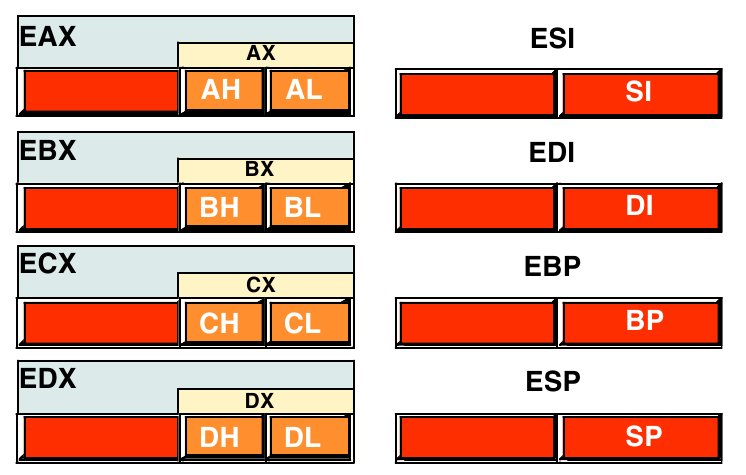
\includegraphics[height=1.6in]{images/registers.jpeg}
        \label{Registers Division}
      \end{figure}
    \end{column}
    \begin{column}{2.5in}
      \begin{itemize}
      \item The register naming system is from IA-16 where the
        registers were called AX, BX, CX, DX.
      \item the ``\texttt{E}'' indicates extended (32 bits). Without
        it, we consider the corresponding 16-bits register
      \item \textbf{Memorandum:} although we are in IA-32
        \begin{itemize}
        \item byte (8 bits)
        \item word (2 bytes)
        \item dword (double word, 4 bytes)
        \end{itemize}
      \end{itemize}
    \end{column}
  \end{columns}
\end{frame}

\begin{frame}
  \frametitle{(1) What about EFLAGS?}
  \begin{figure}
    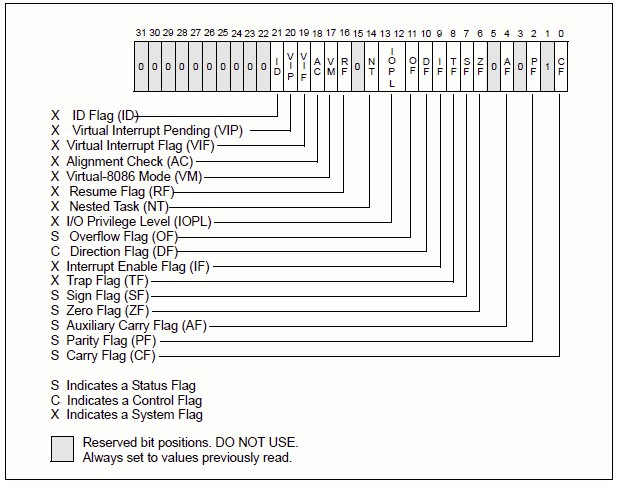
\includegraphics[height=2.5in]{images/eflags.jpeg}
    \label{Eflags idea}
  \end{figure}
\end{frame}
\begin{frame}
  \frametitle{(2) What about EFLAGS?}
  \begin{itemize}
  \item{It's another 32-bits register}
  \item{Only 8 bits out of 32 are of interest for us. The others are either for the kernel mode function or  are of little interest for programmers}
  \item{These 8 bits are called flags. We consider them singularly. They are boolean (true/false) }
  \item{They represent overflow, direction, interrupt disable, sign, zero, auxiliary carry, parity and carry flags}
  \item{Since they represent information about the instruction last executed, they change at every execution step. They are VERY important for the control flow of the program}
  \end{itemize}
\end{frame}


\subsection{Overview on Assembly}
\begin{frame}
  \frametitle{Assembly}
  \begin{itemize}
  \item{Low-Level Language}
  \item{Directly mapped with binary code}
  \item{Custom per Architecture ({\bf x86}, PowerPC, ARM ...)}
  \end{itemize}
\end{frame}

\begin{frame}
  \frametitle{Syntax}
  \begin{itemize}
  \item{In the assembly world we can find two main syntaxes: AT\&T and Intel}
  \item{AT\&T syntax is used by all UNIX program (e.g., \texttt{gdb} by default)}
  \item{Intel syntax is used by Microsoft programs (IDApro and others)}
  \end{itemize}
\end{frame}

\begin{frame}{(1) Differences in the notation}
  \begin{itemize}
  \item{Consider the following operation:\newline
      \centerline{``move the value 0 to EAX''}}
  \item{AT\&T: \centerline{\texttt{mov \$0x0,\%eax}} }
  \item{Intel: \centerline{\texttt{mov eax, 0h}}}
    \item{Main differences:}
      \begin{itemize}
      \item{In AT\&T syntax the destination is the second operand, and vice-versa in Intel syntax}
      \item{In AT\&T syntax registers are denoted with \texttt{\%} and immediates (i.e., costants) with \$. In the Intel syntax these tokens are not used. }
      \end{itemize}
    \end{itemize}
  \end{frame}

\begin{frame}
  \frametitle{(2) Differences in pointer de-referencing}
  \begin{itemize}
  \item{Consider this new operation:\newline\centerline {"move the value 0 to the address contained in EBX+4"}}
  \item{AT\&T: \centerline{ \texttt{mov \$0x0,0x4(\%ebx)}}}
  \item{Intel: \centerline{ \texttt{mov [ebx+4h],0h} }}
  \item{Main differences:}
    \begin{itemize}
    \item{Parentheses: round vs. square}
    \item{Offsets: out and before vs. inside with a \texttt{`+'} sign}
    \end{itemize}
  \end{itemize}
\end{frame}
\subsection{Basic Instructions}
\begin{frame}
  \frametitle{(1) Basic instructions overview}
  \begin{itemize}
  \item{Every processor has a large instruction set (see Intel manual\footnote{\url{http://www.intel.com/content/www/us/en/processors/architectures-software-developer-manuals.html}})}
  \item{A subset of the whole instruction set is usually processor dependent}
  \item{We will focus on the subset of instructions that is common among the processors}
  \item{We will use the Intel syntax as it is the same syntax used in IDApro by default}
  \item Very good reference: \url{http://ref.x86asm.net/geek32.html}
  \end{itemize}
\end{frame}
\begin{frame}
  \frametitle{(2) Basic Instruction MOV}
  \begin{itemize}
  \item{MOV \underline{\textbf{destination}}, \underline{\textbf{source}}}\\
    \textbf{source} can be an immediate, a register, a memory location\\
    \textbf{destination} can be either a register  or a memory location\\

    NB: Every combination except memloc to memloc: It is invalid in
    every instruction!

  \item{Move value from source to destination. There are tons of
      different versions, depending on the operands size (byte, word,
      dword), immediate to reg, immediate to memory, etc. }
  \item{Examples}
    \begin{table}[h]
      \begin{tabular}{|c|c|c|}
        \hline
        MOV eax, ebx&MOV eax, FFFFFFFFh &MOV ax, bx\\    \hline
        MOV [eax],ecx&MOV [eax],[ecx] \color{red}NO!!!&MOV al, FFh\\
        \hline
      \end{tabular}
    \end{table}
  \end{itemize}

\end{frame}
\begin{frame}
  \frametitle{(3) Basic Instruction ADD}
  \begin{itemize}
  \item{ADD \underline{\textbf{destination}}, \underline{\textbf{source}}}\\
    \textbf{source} can be an immediate, a register, a memory location\\
    \textbf{destination} can be either a register or a memory location\\
    NB: The destination has to be at least as large as the source.

  \item{Semantic: destination = destination + source}
  \item{Examples}
    \begin{table}[h]
      \begin{tabular}{|c|c|c|}
        \hline
        ADD esp, 44h&ADD eax, ebx&ADD al, dh\\
        \hline
        ADD  edx, cx&ADD [eax],[ecx] \color{red}NO!!!&ADD [eax],1h\\
        \hline
      \end{tabular}
    \end{table}

  \end{itemize}
\end{frame}
\begin{frame}
  \frametitle{(4) Basic Instruction SUB}
  \begin{itemize}
  \item{SUB \underline{\textbf{destination}}, \underline{\textbf{source}}}\\
    \textbf{source} can be an immediate, a register, a memory location\\
    \textbf{destination} can be either a register or a memory location\\
    NB: The destination has to be at least as large as the source.
  \item{Semantic: destination = destination - source}

  \item{Examples}
    \begin{table}[h]
      \begin{tabular}{|c|c|c|}
        \hline
        SUB esp, 33h&SUB eax, ebx&SUB al, dh\\
        \hline
        SUB edx, cx&SUB [eax],[ecx] \color{red}NO!!!&SUB [eax],1h\\
        \hline
      \end{tabular}
    \end{table}

  \end{itemize}
\end{frame}
\begin{frame}
  \frametitle{(5) Basic Instruction MUL}
  \begin{itemize}
  \item{MUL \underline{\textbf{Operand}}}\\
    \textbf{Operand} can be an immediate, a register, a memory location\\

  \item{Multiplies \textbf{Operand} by the value of AL, AX, EAX register, depending on sizeof(Operand)}
    \begin{table}[h]
      \begin{tabular}{|c!{\vrule width 1pt}c|c|c| }
        \hline
        sizeof(Operand):               & 1 byte & 2 bytes& 4 bytes\\

        \hlinewd{1.3pt}

        Other operand                  & AL & AX & EAX\\      \hline
        Most sign. part of result in:  & AH & DX & EDX\\ \hline
        Least sign. part of result in: & AL & AX & EAX\\
        \hline
      \end{tabular}
    \end{table}

  \item{Examples}
    \begin{table}[h]
      \begin{tabular}{|c!{\vrule width 1pt}c|c|c|}
        \hline
        sizeof(Operand):&1 byte & 2 bytes & 4 bytes\\ \hlinewd{1.3pt}

        Immediate&MUL 44h & MUL 4455h & MUL 44556677h\\ \hline
        Register&MUL cl & MUL dx & MUL ebx \\
        \hline
      \end{tabular}
    \end{table}
  \end{itemize}
\end{frame}

\begin{frame}
  \frametitle{(6) Basic Instruction DIV}
  \begin{itemize}
  \item{DIV \underline{\textbf{Operand}}}\\
    \textbf{Operand} can be an immediate, a register, a memory location

  \item{Divides the value in the dividend register(s) by Operand}
    \begin{table}[h]
      \begin{tabular}{|c!{\vrule width 1pt}c|c|c| }
        \hline
        sizeof(Operand): & 1 byte & 2 bytes & 4 bytes\\	\hlinewd{1.3pt}
        Dividend     & AX     & DX:AX   & EDX:EAX\\	\hline
        Remainder  & AH & DX & EDX\\		\hline
        Quotient  & AL & AX & EAX\\							\hline
      \end{tabular}
    \end{table}
  \item{Examples}
    \begin{table}[h]
      \begin{tabular}{|c!{\vrule width 1pt}c|c|c|}
        \hline
        sizeof(Operand):&1 byte & 2 bytes & 4 bytes\\ \hlinewd{1.3pt}
        Register&DIV bl & DIV bx & DIV ebx\\ \hline
        Immediate&DIV 66h & DIV 6677h & DIV 66778899h \\
        \hline
      \end{tabular}
    \end{table}
  \end{itemize}
\end{frame}

\begin{frame}
  \frametitle{(7) Control-flow Instruction CMP}
  \begin{itemize}
  \item{CMP \underline{\textbf{Operand\_1}}, \underline{\textbf{Operand\_2}}}\\

  \item{Operand\_1 minus Operand\_2 subtraction and sets the flags (ZF,CF,OF, etc.), it doesn't store the result}
  \item{Examples}
    \begin{table}[h]
      \begin{tabular}{|c|c|c|}
        \hline
        CMP eax, ebx&CMP eax, 44BBCCDDh&CMP al, dh\\
        \hline
        CMP al, 44h&CMP ax,FFFFh&CMP [eax],4h\\
        \hline
      \end{tabular}
    \end{table}
  \end{itemize}
\end{frame}
\begin{frame}
  \frametitle{(8) Control-flow Instruction JMP}
  \begin{columns}
    \begin{column}{0.4\columnwidth}
      \begin{figure}
        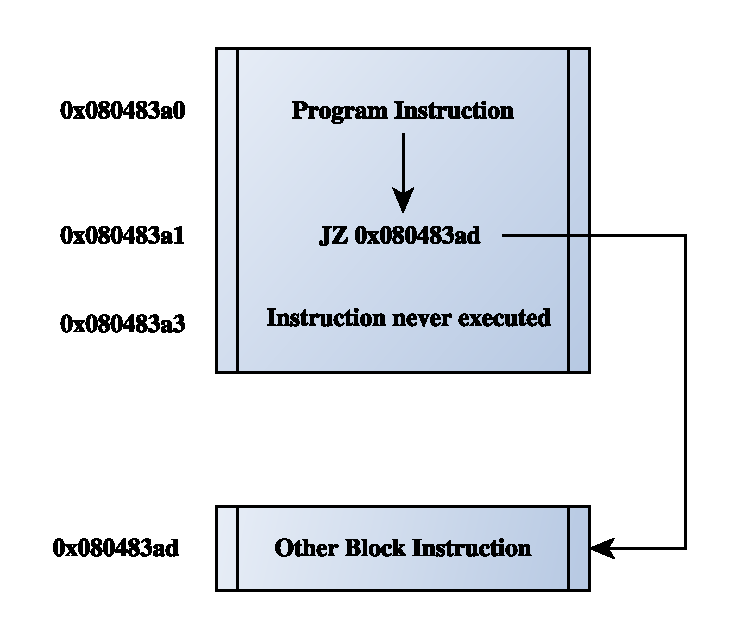
\includegraphics[width=1.2\textwidth]{images/jmp.eps}

        \label{Control Flow JMP}
      \end{figure}
    \end{column}
    \begin{column}{0.6\columnwidth}
      \begin{itemize}
      \item{JMP \underline{\textbf{address}} or \underline{\textbf{offset}}}\\

      \item{Called ``unconditional jump'': sets the EIP to the address. We say that the execution ``jumps to \textbf{address}'' and it's unconditional because it always happens.}
      \item{Using an \textbf{offest} the current EIP is incremented (or decreased) by the constant expressed by the \textbf{offest} resulting in a relative jump.}
      \end{itemize}
    \end{column}
  \end{columns}
\end{frame}
\begin{frame}
  \frametitle{(9) Other Control-flow Instructions: JZ, JNZ and so on}
  \begin{columns}
    \begin{column}{2.5in}
      \begin{itemize}
      \item{General: J\textbf{X} \underline{\textbf{address}} or \underline{\textbf{offset}}}\\
        $ \mathbf{X} \in \{O,NO,S,NS,E,Z,NE...\}$\\
      \item{These are called ``conditional jumps''}
      \item {The execution will go to \textbf{address} if and only if
          the specific flag of the condition is verified.}
      \item {For example: JZ jumps if and only if ZF (zero flag) is 1}
      \item{\textbf{Offset} is used for relative position (as in JMP)}
      \end{itemize}
    \end{column}\footnote{\url{http://www.unixwiz.net/techtips/x86-jumps.html}}
    \begin{column}{2.5in}
      \begin{figure}
        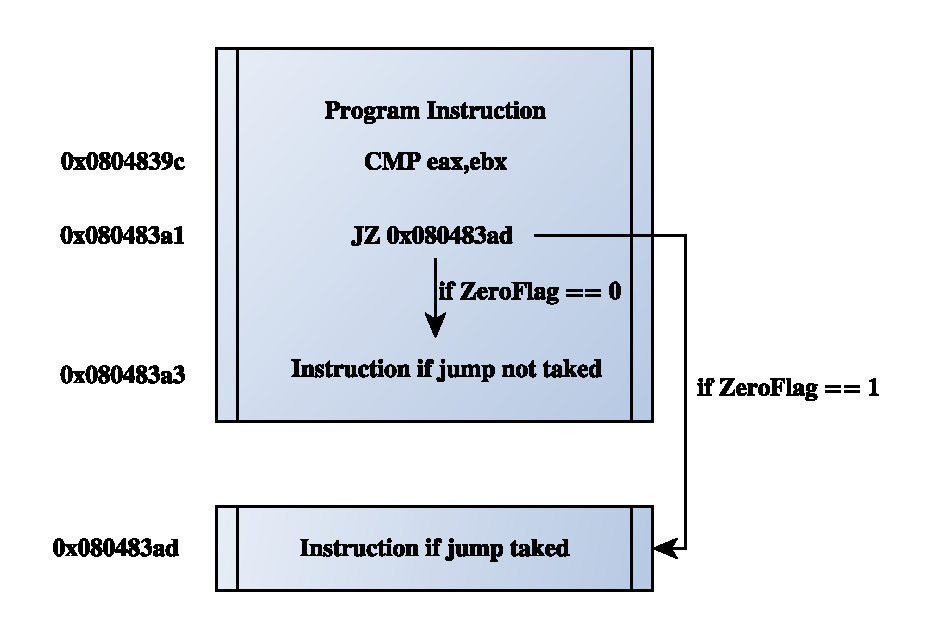
\includegraphics[width=\textwidth]{images/j_unc.eps}									      \label{control}
        \label{Control Flow JZ}
      \end{figure}
    \end{column}

  \end{columns}
\end{frame}

\begin{frame}
  \frametitle{(10) Basic Instruction NOP}
  \begin{itemize}
  \item{NOP}\\
  \item{The meaning of NOP is \textbf{No Operation}. Just move to next instruction.}
  \item{The opcode is pretty famous and is \textbf{0x90}}
  \item{Really useful in exploitation (we will see).}
  \end{itemize}
\end{frame}


\begin{frame}
  \frametitle{(11) Basic Instruction INT}
  \begin{itemize}
  \item{INT \underline{\textbf{VALUE}}}\\
  \item{\textbf{VALUE} is the software interrupt number to generate (0-255)}
  \item{Famous values are 21h for call service under Windows and 80 for Linux}
  \item{Every OS has its set of interrupt numbers}
  \end{itemize}
\end{frame}


\begin{frame}
  \frametitle{(12) Syscall/SYSENTER}
  Nowadays Syscalls are done with specific instructions.
  \begin{itemize}
  \item{syscall is used for Linux 64-bit}
  \item{SYSENTER is used by Microsoft Windows}
  \end{itemize}
\end{frame}

\subsection{x86\_64}
\begin{frame}
  \frametitle{How much is x86\_64 different from x86?}
  \begin{changemargin}{-0.7cm}{0cm}
    \begin{itemize}
    \item{The prefix of  the registers is R instead of E so we have ({\bf RIP}, {\bf RAX} etc.)}
    \item{There are 8 new registers ({\bf R8} to {\bf R15})}
    \item{each of them can be considered at 8, 16, 32, 64 bits (qword)\\
        with $X \in \{8..15\}$ we have }
      \begin{table}[h]
        \begin{tabular}{|c!{\vrule width 1pt }c|c|c|c|}
          \hline
          bits&8&16&32&64\\
          \hline
          reg&rXb&rXw&rXd&rX\\
          \hline
        \end{tabular}
      \end{table}
    \item{for better syntax information look at \url{http://www.x86-64.org/documentation/assembly.html}}
    \end{itemize}
  \end{changemargin}
\end{frame}
\section{Something more}

\subsection{Program Layout In Memory}

\begin{frame}
  \frametitle{Binary File Formats}
  \begin{itemize}
  \item{\textbf{PE (Portable Executable):} used by Microsoft binary executable.}
  \item{\textbf{ELF:} common binary format for Unix, Linux, FreeBSD and others}
  \item In both cases, we are interested in how each executable is
    mapped into memory, rather than how it is organized on disk.
  \end{itemize}
\end{frame}

\begin{frame}
  \begin{changemargin}{-1cm}{-1cm}
    \frametitle{How an executable is mapped to memory in Linux (ELF)}
    \begin{table}[l]
        \scalebox{0.7}{

          \begin{tabular}{|l l|}
            \hlinewd{1pt}
            \textbf{Executable}&\textbf{Description}\\\hlinewd{1.3pt}
            .bss&This section holds uninitialized data that contributes to the program's memory image.\\
            &By definition, the system initializes the data with zeros when the program begins to run.\\\hline
            .comment&This section holds version control information.\\\hline
            .data/.data1& These sections hold initialized data that contribute to \\
            &the program's memory image\\\hline
            .debug&This section holds information symbolic debugging.\\\hline
            .text&This section holds the "text," or executable instructions, of a program.\\\hline
            .init&This section holds executable instructions that contribute to the process initialization code.\\
            &That is, when a program starts to run, the system arranges to execute the code in this\\
            &section before calling the main program entry point (called main for C programs).\\
            \hline
            .got&This section holds the global offset table.\\
            \hline

          \end{tabular}
      }
    \end{table}
  \end{changemargin}
\end{frame}

\begin{frame}
  \begin{changemargin}{-1cm}{-1cm}
    \frametitle{How an executable is mapped to memory in Windows (PE)}
    \begin{table}[l]
        \scalebox{0.9}{
          \begin{tabular}{|l l|}
            \hlinewd{1pt}
            \textbf{Executable}&\textbf{Description}\\\hlinewd{1.3pt}
            .text&Contains the executable code\\\hline
            .rdata&Holds read-only data that is globally accessible within	\\
            &the program\\\hline

            .data&Stores global data accessed throughout the program\\\hline
            .idata&stores the import function information;\\\hline
            .edata&stores the export function information;\\\hline
            .pdata&Present only in 64-bit executables and stores\\
            & execption-handling information\\\hline
            .rsrc&Stores resources needed by the executable\\\hline
            .reloc&Contains information for relocation of library files\\\hline
          \end{tabular}
      }
    \end{table}
  \end{changemargin}
\end{frame}

\begin{frame}
  \frametitle{A more realistic view of an elf in memory}
  \begin{center}
    {\tiny Low addresses (0x80000000)}
    \begin{center}
      \begin{tikzpicture}[every
        node/.style={font=\ttfamily\footnotesize}]
        \node [stack,rectangle split parts=8] (s) {%
          Shared libraries%
          \nodepart{two}%
          .text%
          \nodepart{three}%
          .bss%
          \nodepart{four}%
          heap \textrm{(grows $\downarrow$)}%
          \nodepart{five}%
          ...%
          \nodepart{six}%
          stack \textrm{(grows $\uparrow$)}%
          \nodepart{seven}%
          env%
          \nodepart{eight}%
          argc%
        };
      \end{tikzpicture}
    \end{center}
    {\tiny High addresses (0xbfffffff)}
  \end{center}
\end{frame}

\begin{frame}
  \frametitle{The stack}
  \begin{itemize}
  \item{Last In First Out (LIFO) data structure: the most recent data placed, or pushed, onto the stack is the first item to be removed, or popped, from it}
  \item{A LIFO is ideal for storing transitory data, or data that does not need to be stored for long.}
  \item{The stack stores local variables, information related to function calls or used to clean up the stack after a function or procedure returns.}
  \item{Remember: the stack grows downward the address space, toward lower addresses.}
  \end{itemize}
\end{frame}
\begin{frame}
  \frametitle{Stack Management Instruction: PUSH}
  \begin{itemize}
  \item{Pushes a word onto the stack}
  \item{Example: PUSH {\bf immediate} or PUSH {\bf register} }
  \item{Pushes the immediate or register value at the top of the stack and decrements the ESP of sizeof(immediate or register)}
  \end{itemize}
\end{frame}
\begin{frame}
  \frametitle{Stack Management Instruction: POP}
  \begin{itemize}
  \item{Pops a word from the stack}
  \item{Example: POP {\bf destination} }
  \item{Pops the word off of the top of the stack and moves it at destination, then it increases the ESP of sizeof(data popped).}
  \end{itemize}
\end{frame}


\begin{frame}
  \frametitle{Endianness}
  The \textbf{endianness} is a convention that specifies in which order the bytes of a data word are lined up sequentially in memory.
  \begin{columns}
    \begin{column}{0.72\columnwidth}
      \textbf{Big-endian} (left) systems are systems in which the \emph{most significant byte} of the word is stored in the \emph{smallest address} given.
    \end{column}
    \begin{column}{0.28\columnwidth}
      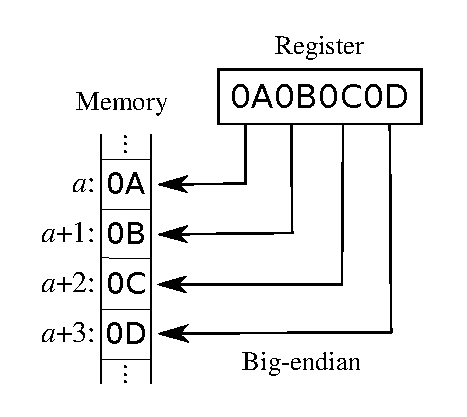
\includegraphics[width=\textwidth]{images/Big-Endian.pdf}
      \label{Big-Endian}
    \end{column}
  \end{columns}
  \begin{columns}
    \begin{column}{0.28\columnwidth}
      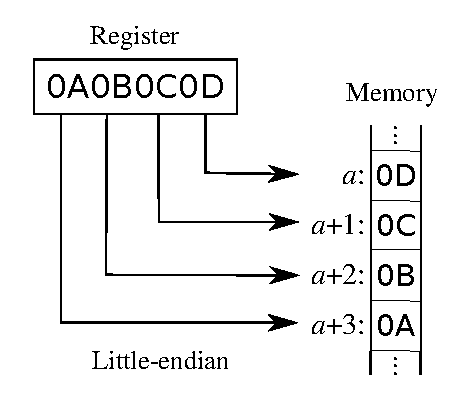
\includegraphics[width=\textwidth]{images/Little-Endian.pdf}
      \label{Little-Endian}

    \end{column}
    \begin{column}{0.72\columnwidth}
      \yellowemph{\textbf{Little-endian} (right)} systems are those in
      which the \emph{least significant} byte is stored in the
      \emph{smallest address}. \yellowemph{A-32 is ``little endian''}.

    \end{column}

  \end{columns}
\end{frame}


\begin{frame}
  \frametitle{Endianness cont.}
  The \textbf{endianness} is a convention that specifies in which order the bytes of a data word are lined up sequentially in memory.
  \begin{columns}
    \begin{column}{0.5\columnwidth}
      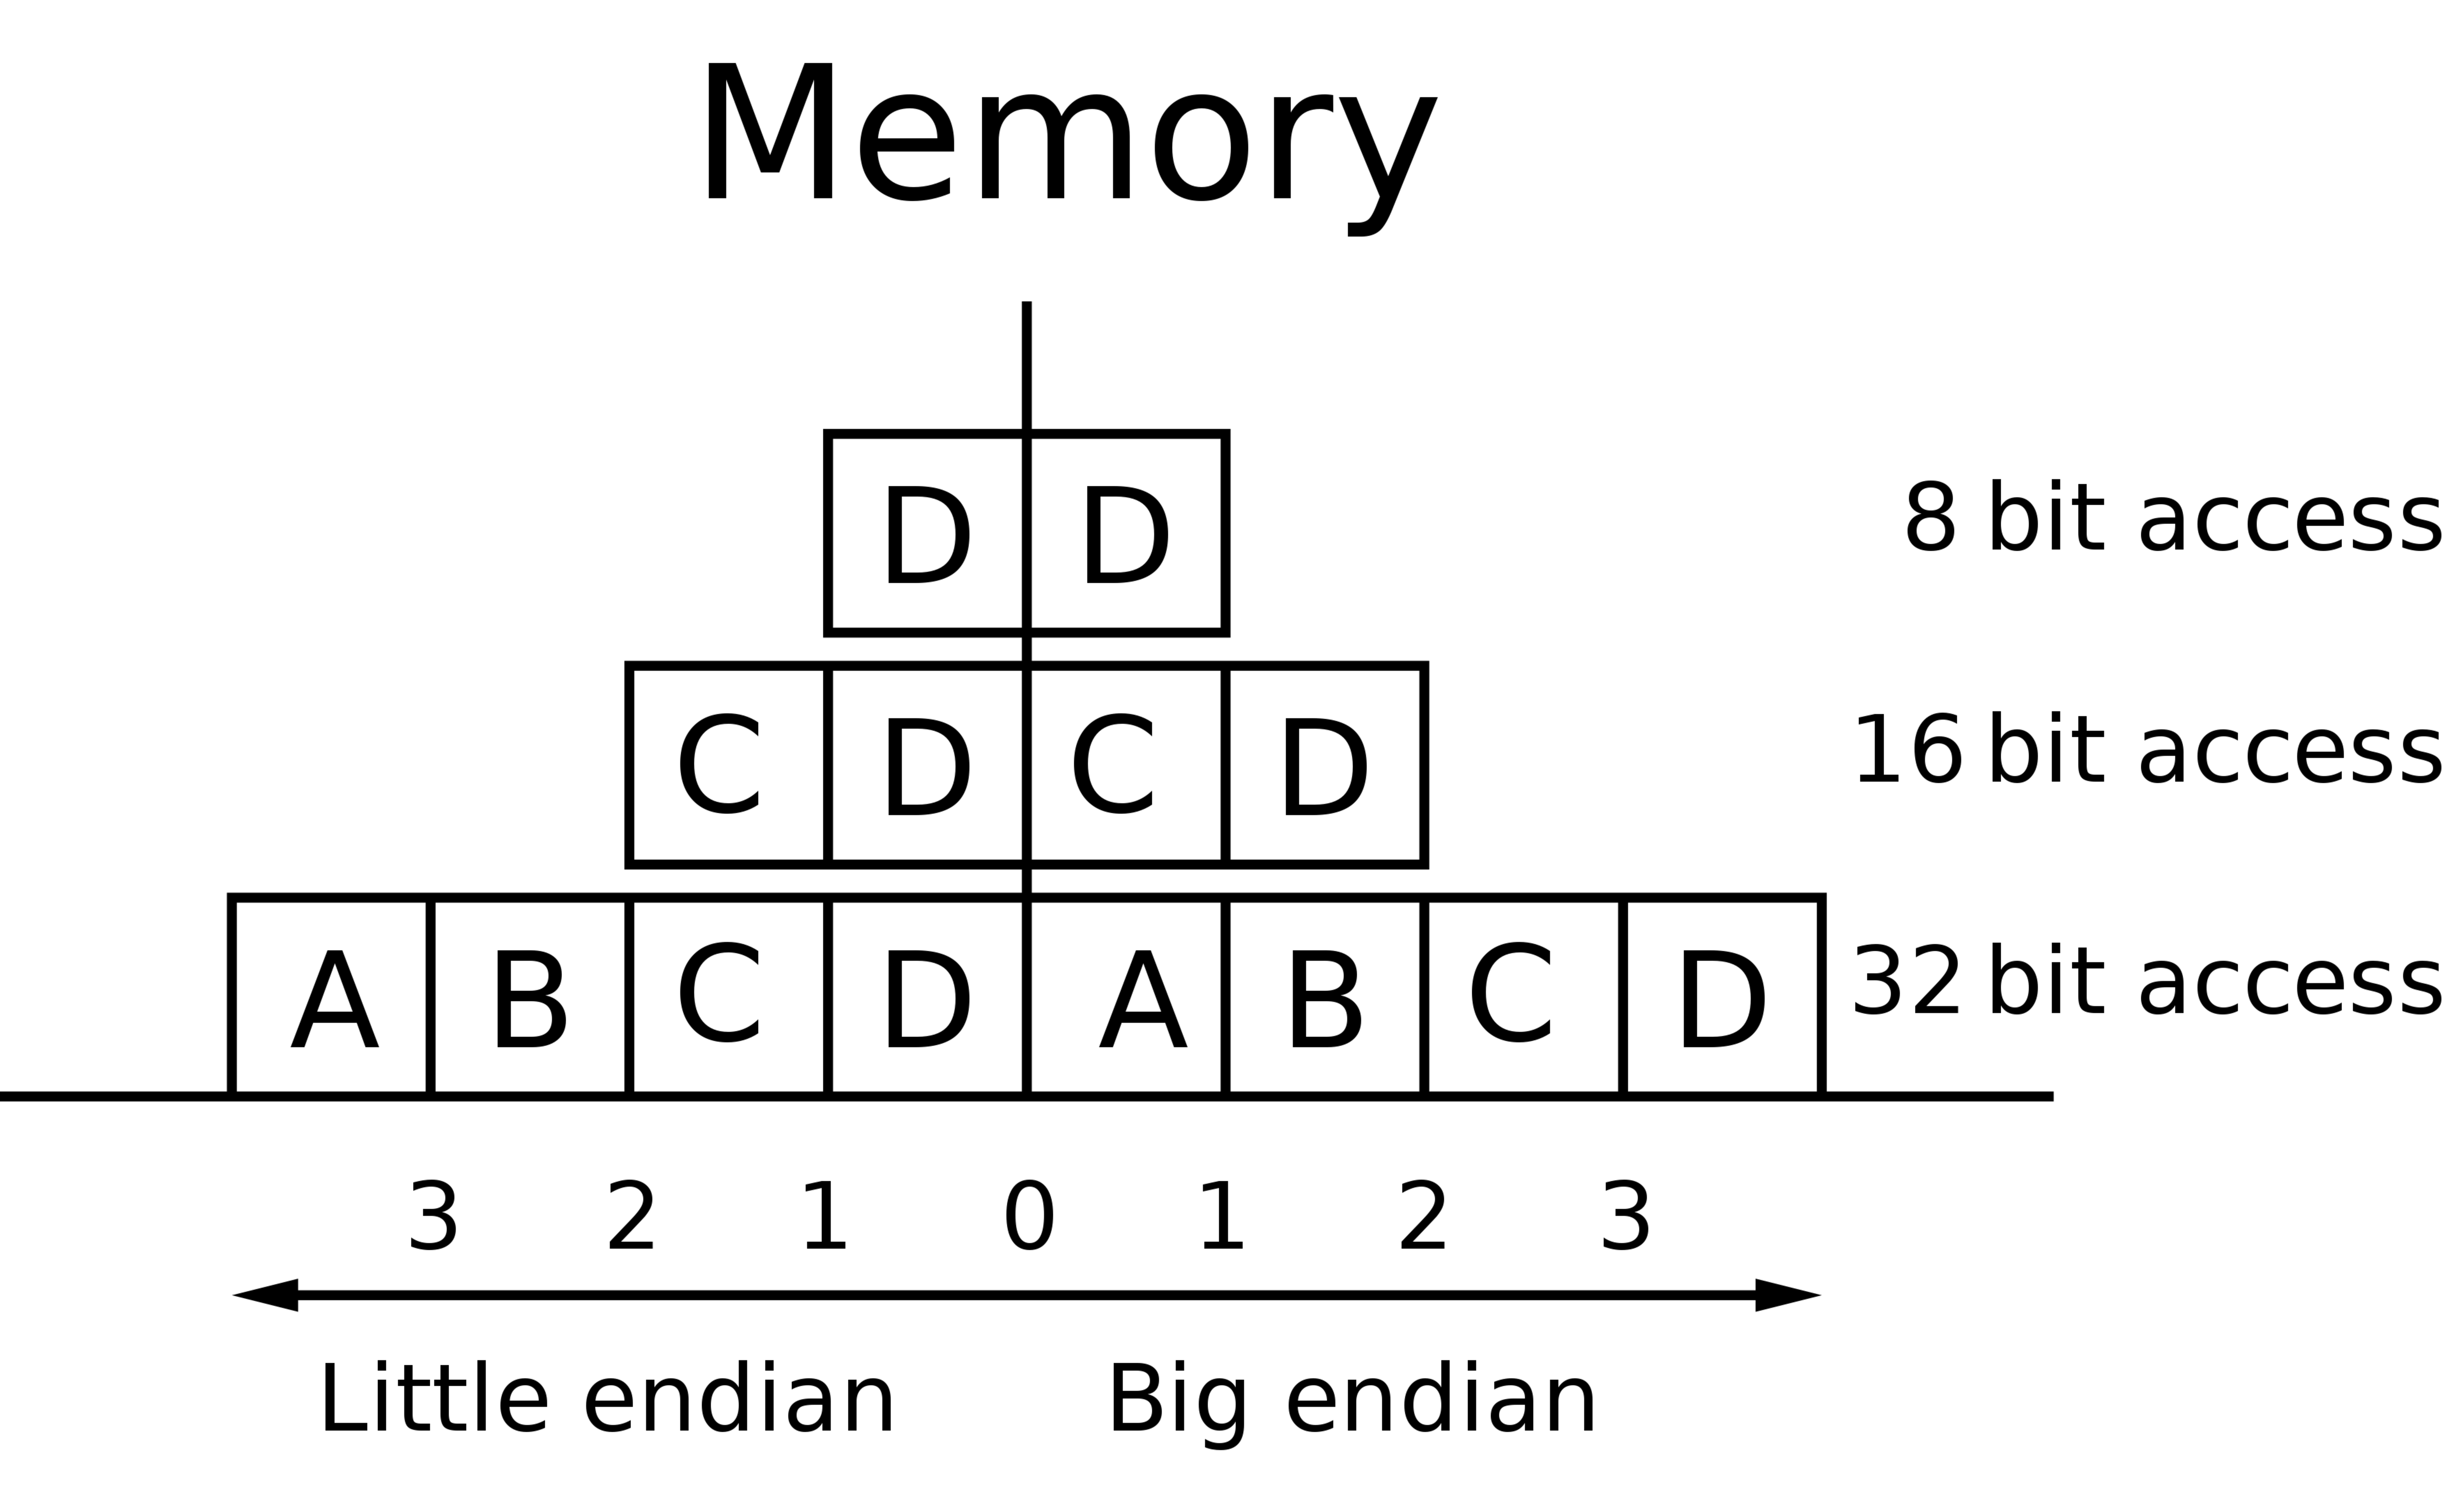
\includegraphics[width=\textwidth]{images/Endianessmap1.pdf}
      \label{Big-Endian}
    \end{column}
    \begin{column}{0.5\columnwidth}
      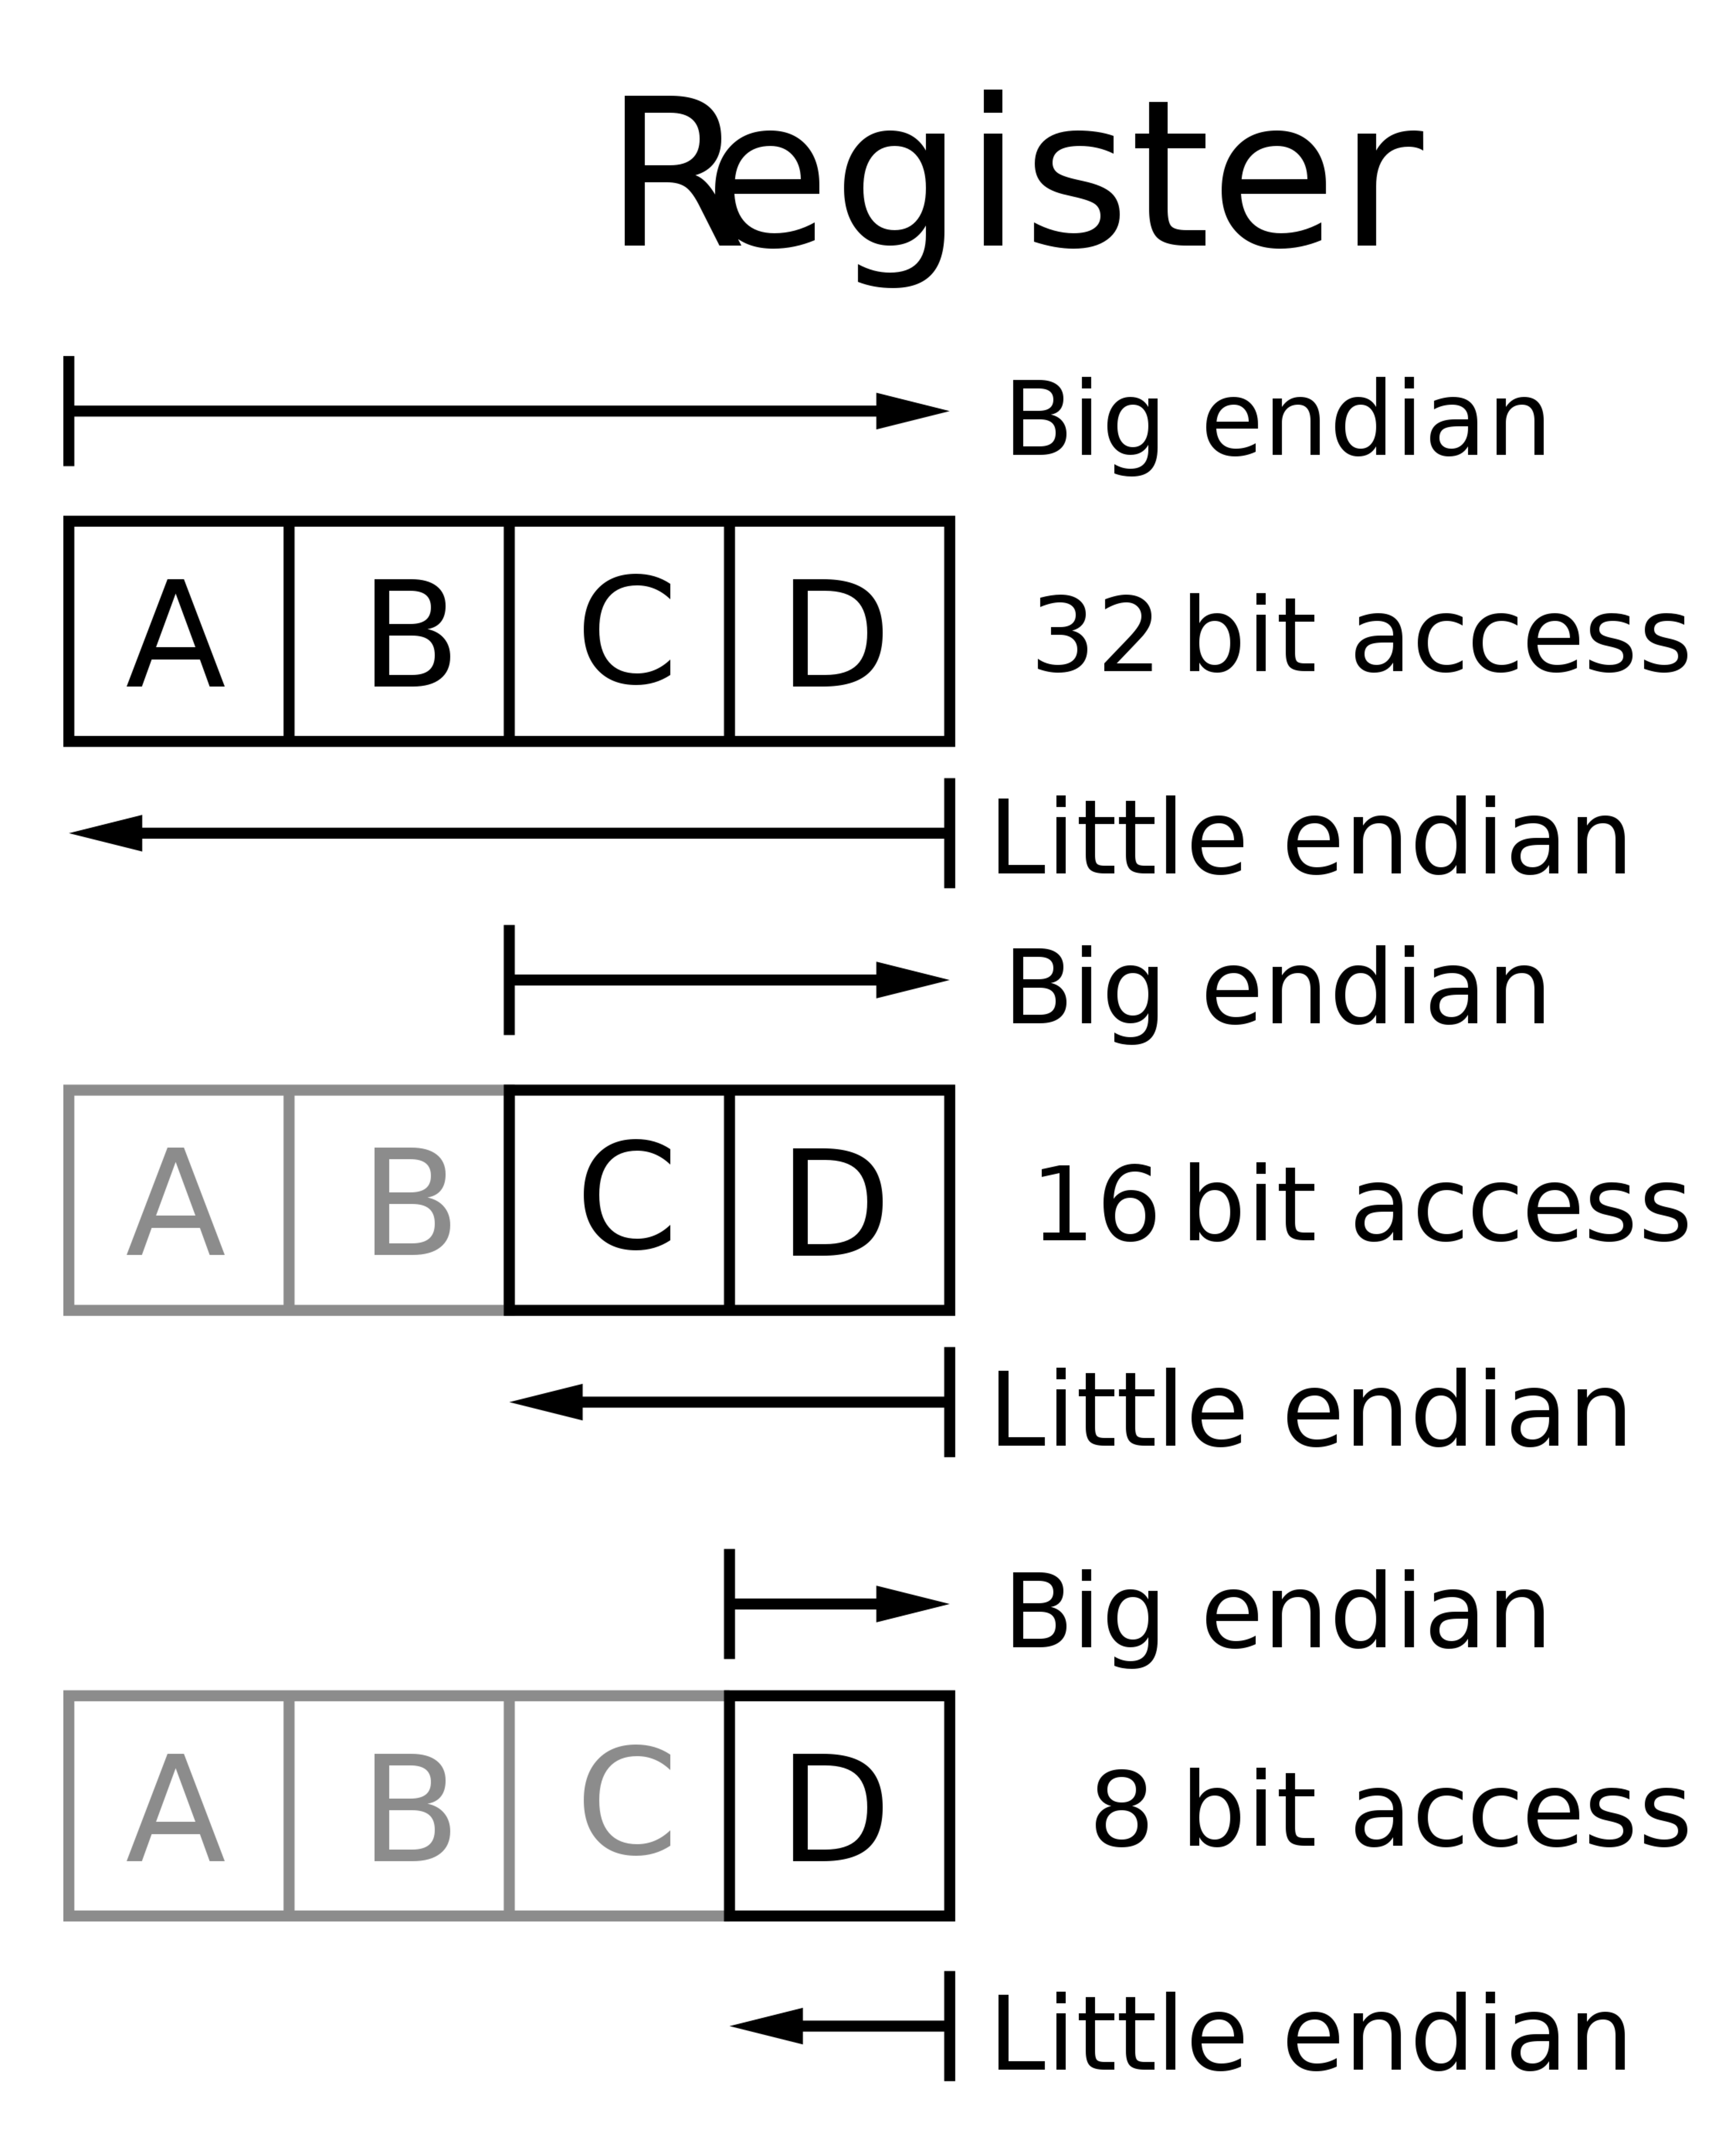
\includegraphics[width=0.6\textwidth]{images/Endianessmap2.pdf}
      \label{Little-Endian}
    \end{column}
  \end{columns}
\end{frame}



\subsection{Functions and Calling Convention}
\begin{frame}
  \frametitle{Functions}
  \begin{itemize}
  \item{The concept of {\it ``function''} at the machine level is the same as in high-level programming languages}
  \item{{\bf Function}: piece of code that receives data from the caller, execute code and returns some value}
  \item{{\bf Calling convention}: how parameters are passed and value is retured = which instructions are executed to do this}
  \item{There exist several calling conventions, depending on architecture, OS and binary format}
  \end{itemize}
\end{frame}

\begin{frame}
  \frametitle{CALL and RET Instruction}
  \begin{itemize}
  \item{CALL {\bf func} changes the exectuion flow to the {\bf func} location. It stores return address of the instruction after the call onto the stack and moves into EIP the address of the first instruction of {\bf func}} (PUSH EIP; JMP func;)
  \item{RET {\bf value} returns to the previous function (i.e., caller). It restores return address saved by the CALL.} (POP EIP;)
  \end{itemize}
\end{frame}

% \begin{frame}
%   \frametitle{Functions: An example as seen in IDAPro}
%   \begin{figure}
%     \scalebox{0.54}{
%       \includegraphics[width=\textwidth]{images/function.eps}
%       \label{A Function Example}
%     }
%   \end{figure}
% \end{frame}

\begin{frame}
  \frametitle{Calling Convention}
  \begin{itemize}
  \item{How a function receives parameters and returns the value and how it administers the stack}
  \item{There are several calling conventions that dictate where a caller should place any parameters that a function requires}
  \item{The high-level language, the compiler, the OS, and the target architecture all together ``implement'' and ``agree upon'' a certain calling convention.}
  \item{Let's look at some examples}
  \end{itemize}
\end{frame}

\begin{frame}
  \frametitle{The C Calling Convention}
  \begin{itemize}
  \item{It's the default calling convention used by most C compilers for the x86 architecture}
  \item{When a compiler doesn't use this convention we can force it using the modifier \color{red}\_cdecl}
  \item{It specifies that the \textbf{caller places} parameters on the stack in the right to left order and that the \textbf{caller removes} the parameters from the stack after the called function completes}
  \end{itemize}
\end{frame}
\begin{frame}[fragile]
  \frametitle{The C Calling Convention example}
\begin{lstlisting}[language=C]
void demo_cdecl(int a, int b, int c, int z);

//...

demo_cdecl(1, 2, 3, 4); //calling
\end{lstlisting}

\begin{lstlisting}[language={[x86masm]Assembler}]
; ...
push 4          ; push last parameter value
push 3          ; push third parameter value
push 2          ; ...
push 1
call demo_cdecl ; call the subroutine
\end{lstlisting}

\end{frame}

\begin{frame}[fragile]
  \frametitle{The Standard Calling Convention}
  \begin{itemize}
  \item{This is Miscrosoft's calling convention standard}
  \item{When a compiler doesn't use this convention we can force it using the modifier \color{red}\_stdcall}
  \item{The parameters are passed using the stack as in \_cdecl, but in \_stdcall the called function is \textbf{responsible for clearing the function parameters from the stack before returning}. To do this, the function needs to know the right number of parameter passed. Can be used only with functions having a fixed number of parameters (e.g., no \texttt{printf}).}
  \end{itemize}

\begin{lstlisting}[language=C]
void _stdcall demo_stdcall(int a, int b, int c);
demo_stdcall(1, 2, 3);
\end{lstlisting}
\begin{lstlisting}[language={[x86masm]Assembler}]
ret 12  ; return and clear 12 bytes from the stack
\end{lstlisting}
\end{frame}

\begin{frame}[fragile]
  \frametitle{fastcall Convention for x86}
  \begin{itemize}
  \item{Variation of the standard calling convention}
  \item {passes up to 2 parameters via registers (faster than stack).}
  \item{The Microsoft Visual C/ C++ and GNU GCC/g++ compilers recognize the \color{red}fastcall \color{black} modifier in function declaration.}
  \item{Example: the 1st and 2nd parameters are passed via ECX and EDX, the remainder parameters pushed on the stack in right to left order. The called function must cleanup the stack when returning.}
  \end{itemize}
\begin{lstlisting}[language={[x86masm]Assembler}]
; demo_fastcall(1, 2, 3, 4);
push 4 ; push 4th parameter
push 3 ; push 3rd parameter
mov edx, 2 ; move 2nd parameter in EDX
mov ecx, 1 ; move 1st parameter in ECX
call demo_fastcall
\end{lstlisting}
\end{frame}

\begin{frame}[fragile]
  \frametitle{A Closer Look at the cdecl Calling Convention}
  \begin{columns}
    \begin{column}{.5\textwidth}
\begin{lstlisting}[language=C]
void function (int a, int b) {
  int array [5];
}

int main (int argc, char** argv) {
  function(1, 2);
  printf("This is where the ret address points");
}
\end{lstlisting}
    \end{column}
    \begin{column}{.5\textwidth}
      \begin{center}
        {\tiny Low memory addresses (top of the stack)}
        \begin{center}
          \begin{tikzpicture}[every
            node/.style={font=\ttfamily\footnotesize}]
            \node [stack,rectangle split parts=7] (s) {%
              ...%
              \nodepart{two}%
              array[0]%
              \nodepart{three}%
              Saved EBP%
              \nodepart{four}%
              return address%
              \nodepart{five}%
              1%
              \nodepart{six} 2%
              \nodepart{seven}%
              ...  };
          \end{tikzpicture}
        \end{center}
        {\tiny High memory addresses (bottom of the stack)}
      \end{center}

    \end{column}
  \end{columns}
\end{frame}

\begin{frame}[fragile]
  \frametitle{Assembler-level View of the Same Example}
  \begin{columns}
    \begin{column}{.5\textwidth}

\begin{lstlisting}[language={[x86masm]Assembler},basicstyle=\tiny\ttfamily]
public main
main proc near
push ebp
mov ebp, esp ; create stack
and esp,0FFFFFFFF0h
sub esp,10h ; make room for vars
mov dword ptr[esp+4],2 ; push 2
mov dwrod ptr[esp],1 ; push 1
call function
mov dword ptr [esp], offset format; "This is..."
call _printf
leave
ret
main endp

public function
function proc near
push ebp
mov ebp,esp ; create stack
sub esp,20h ; make room for array
leave
retn 8 ; remove 2 dwords
function endp
\end{lstlisting}
    \end{column}

    \begin{column}{.5\textwidth}

      \begin{center}
        {\tiny Low memory addresses (top of the stack)}
        \begin{center}
          \begin{tikzpicture}[every
            node/.style={font=\ttfamily\footnotesize}]
            \node [stack,rectangle split parts=7] (s) {%
              ...%
              \nodepart{two}%
              array[0]%
              \nodepart{three}%
              Saved EBP%
              \nodepart{four}%
              return address%
              \nodepart{five}%
              1%
              \nodepart{six} 2%
              \nodepart{seven}%
              ...  };
          \end{tikzpicture}
        \end{center}
        {\tiny High memory addresses (bottom of the stack)}
      \end{center}
    \end{column}
  \end{columns}
  \begin{figure}
  \end{figure}
\end{frame}

\subsection{objdump -- GDB tutorial}
\begin{frame}
  \frametitle{Objdump}
  \begin{itemize}
  \item{{\bf man objdump}}\\
objdump \textbf{displays information} about one or more \textbf{object files}.
  \item{\textbf{-x}} all-headers
  \item{\textbf{-d}} disassemble
  \item{\textbf{-M intel}} intel syntax (default is att)
  \end{itemize}
\end{frame}

\begin{frame}
  \frametitle{Our friend gdb}
  \begin{itemize}
  \item{{\bf What is GDB?}}\\
    GDB is GNU Project's Debugger: allows to follow, step by step, at assembler-level granularity, a running program, or what a program was doing right before it crashed.\footnote{http://www.gnu.org/software/gdb/}
  \end{itemize}
\end{frame}

\begin{frame}
  \frametitle{Start, break and navigate the execution with gdb}
  \begin{itemize}
  \item{Suppose you have an executable binary and want run it}\\
    \begin{itemize}
    \item{{\bf gdb /path/to/executable} loads the binary in gdb}
    \end{itemize}
  \item{Now you decide to start the program with two parameters}\\
    \begin{itemize}
    \item{{\bf run 1 "abc"} passes 1 via \path|argv[1]| and
        \path|"abc"| as \path|argv[2]|}
    \item \textbf{run `printf "AAAAAAAAAAAA"`} (with the back ticks)
      we're passing the output of the print (very useful when you need
      to pass non printable characters such as raw bytes)
    \end{itemize}
  \item{Suppose you want to stop the execution at the address of a
      certain instruction}
    \begin{itemize}
    \item{{\bf break *0xDEADBEAF} places a break point at that address}
    \item{{\bf break *main+1} with debugging symbols this can be less painful}
    \item{{\bf catch syscall} block the execution when a syscall happens}
    \end{itemize}
  \end{itemize}
\end{frame}

\begin{frame}
  \frametitle{Start, break and navigate the execution with gdb}
  \begin{itemize}
  \item{Now the execution stops at our break point. Here we
      can do several things}
  \item{Examples:}
    \begin{itemize}
    \item{{\bf ni} allows to procede instruction per instruction}
    \item{{\bf next 4} moves 4 lines ahead (if you have the
        line-numbers information in the binary)}
    \item{{\bf si} step into function}
    \item{{\bf finish} run until the end of current function}
    \item{{\bf continue} runs until the next break point (if any)}

    \end{itemize}
  \item{To see info about the execution state:}
    \begin{itemize}
    \item{{\bf info registers} to inspect the content of the registers}
    \item{{\bf info frame} to see the values of the stack frame
        related to the function where we are in}
    \item{{\bf info file} print the information about the sections of the binary}
    \end{itemize}
  \end{itemize}
\end{frame}

\begin{frame}
  \frametitle{Navigate the stack}
  \begin{itemize}
  \item{Suppose we're stopped somewhere in the code and want to
      inspect the stack}
  \item{Some useful view of the stack is achievable with:}
    \begin{itemize}
    \item{{\bf x/100wx \$esp} prints 100 words of memory from the address found in the ESP to ESP+100 (x = hexadecimal formatting)}
    \item{{\bf x/10wo \$ebp-100} prints 10 words of memory from EBP-100 to EBP-100+10 (o = octal formatting)}
    \item{{\bf x/s \$eax} prints the elements pointed by EAX (s = string formatting)}
    \end{itemize}
  \item{Do you have debug symbols? (i.e., \texttt{gcc -ggdb})}
    \begin{itemize}
    \item{{\bf print args} prints info about the main parameters}
    \item{{\bf print a} prints the content of variable `a'}
    \item{{\bf print *b} prints the value pointed by `b'}
    \end{itemize}
  \end{itemize}
\end{frame}
\begin{frame}
  \frametitle{Our friend gdb}
  \begin{itemize}
  \item{{\bf The '$\sim$/.gdbinit' file}}\\
    Gdb is a command line tool and it supports the configuration script as almost all the *nix software.

    Some options that you may want to tune are:
    \begin{itemize}
    \item{{\bf set history save on}}\\
      To have the lastest commands always available also when we re-open gdb
    \item{{\bf set follow-fork-mode child}}\\
      Allows you, if the process spawns children, to follow them and not only wait their end.
    \item{{\bf set disassembly-flavor [intel \textpipe{}  att]}}\\
      This option sets in which predefined syntax your disassembled will be showed up. The default one is at\&t
    \end{itemize}
  \item Highly recommended to put this
    \url{https://github.com/gdbinit/Gdbinit} file in \path|~/.gdbinit|
  \end{itemize}
\end{frame}

\begin{frame}
  \frametitle{Layout in gdb}
  \begin{itemize}
  \item{You're not a big fun of the gdb command line?}
  \item{Give a simple text-based interface to it}
    \begin{itemize}
    \item{{\bf layout asm} turn the interface to the assembly view always visible during debugging}
    \item{{\bf layout src} if your binary has the dubugging symbols you will have your c source view visible}
    \item{{\bf layout reg} add to the interface the register status view. It could be used in combination with one of the view described above}
    \item{{\bf gdb -tui ./mybin} runs gdb directly in this Text User Interface}
    \end{itemize}
  \item{Use {\bf CTRL+X A} to go back to standard interface.}
  \end{itemize}
\end{frame}

\subsection{Conclusion}
\begin{frame}
  \frametitle{Bibliography}
  \begin{itemize}
  \item The Ida Pro Book 2 Edition
  \item The Shellcoder Handbook
  \item Reverse Engineering Code with IDA Pro
  \item Secrets of Reverse Engineering
  \item Reverse Engineering for Beginners
  \end{itemize}
\end{frame}

\begin{frame}{End}
  \begin{center}\Large
    That's all folks!

    Time for (more) questions!
  \end{center}
\end{frame}

\end{document}

%%% Local Variables:
%%% mode: latex
%%% TeX-master: t
%%% End:
